There always was a tight relation between the development of cameras and pixel detectors since 1969, when the idea of CCDs, thanks to whom Boyle and Smith were awarded the Nobel Prize in Physics in 2009, revolutionized photography allowing light to be captured electronically instead of on film. 
Even though the CMOS technology was already known when CCDs spread, the costs of productions were too high to allow the diffusion of these sensors for which needed to wait untill 1990s. From that period on, the fast diffusion of CMOS was mainly due to the less cost than CCD, and the less power required for supply. Nowadays CCDs are still prefered over MAPS in astronomy, where the astronomical sources' rate are low enough to cope with tens of \si{ms} for the readout.  

The principal use cases of pixel detectors are particle tracking and imaging: in the former case individual charged particles have to be identified, in the latter instead an image is obtained by the usually un-triggered accumulation of the impinging radiation. 
Also the demands on detectors performance depends on their usage, in particular tracking requires high spatial resolution, fast readout and radiation hardness. 


\section{Tracking in HEP}
    At first the physics world overlooked the CCDs, and all pixel in general, as against the gaseous detector for tracking: there was no need to replace these ones which had a sufficient good resolution (\SI{100}{\um}). Sice 1974, with the measurement of the invariant mass of the \red{j psi} and the affirmation of the quark model, all experiments start to look for better spatial resolutions in order to achieve the possibility of reconstructing short lived particle.  

    Historically, the first pixel detector employed in particle physics was a CCD: it was installed in the spectrometer at the CERN’s Super Proton Synchrotron (SPS) by the ACCMOR Collaboration (Amsterdam, CERN, Cracow, Munich, Oxford, RAL) at mid 1980s, with the pourpose of studing the recently-discovered charm particles.
    The second famous usage of CCDs took place at SLAC in the Large Detector (SLD) during the two years 1996-98. 
    \red{Cosa vedono di così importante da dire che servono i pixel detector?}
    From that period on particle tracking in experiments have been transformed radically: it was mandatory for HEP experiments to build a inner vertex detector. 
    In 1991, the more demanding environments led to the development of hybrid pixel detectors: a dedicated collaboration, RD19, was established at CERN with the specific goal to define a semiconductor micropattern detector with an incorporated signal processing at a microscopic level. 
    In those years a wide set of prototypes of hybrid pixel has been manufactured; among the greatest productions a mention goes to the huge ATLAS and CMS vertex detectors. 
    From the middle of 2013 a second collaboration, RD 53, has been established with the new goal to find a pixel detector suitable for phase II future upgrades of those experiments. Even if the collaboration is specifically focused on design of hybrid pixel readout chips (aiming to \SI{65}{nm} tecnique so that the electronics fits within the pixel area), also other options have been taken in account and many test have been done on MAPS for example. Requirements imposed by HL-LHC will become tigher in time: for example, a dose and radiation of \SI{5}{Mrad} and \si{10 {16}}{NIEL} are exepcted after 5 years of operation. Time resolution, material budget and power consumption are also issues for the upgrade: a time resolution better than \SI{25}{ns} for a bunch crossing frequency of \SI{40}{MHz}, a material budget lower than 2\% and a power consuption lower than  \SI{500}{mW/cm\squared} are required. 

    Amidst the solutions proposed 3D silicon detector, invented by Sherwood Parker in 1995, and MAPS are the most promising. In 3D sensors the electrode is a narrow column of n-type implanted vertically across the bulk instead of being implanted on the wafer's surface. 
    The charge produced by the impinging particle is then drifted transversally within the pixel, and, as the mean path between two electrode can be soufficent low, the trap probability is not an issue. 
    3D pixels have been already proved in ATLAS tracker \red{quando?}. 
    Even if 3D detector are adequately radiation hard, MAPS architecture looked very promising from the beginning: they overcome both the CCDs long reading time and the hybrid problems (I have already explained in section \ref{sec:} the benefits of MAPS). 
    Experiments such as ALICE at LHC and STAR at RHIC have already introduced the CMOS MAPS technology in their detectors. ALICE Tracking System (ITS2), upgraded during the LHC long shut down in 2019-20, was the first large-area ($\sim$10 \si{m\squared} covered by 2.5 Gpixels) silicon vertex detector based on CMOS MAPS.

    \subsection{Hybrid pixels at LHC: ATLAS, CMS and LHC-b}
        \subsubsection{ATLAS}    
        With CMS, ATLAS is one of two general-purpose detectors at the LHC and has the largest volume detector ever constructed for a particle
        collider (\SI{46}{m} long and \SI{25}{m} in diameter).  
        The Inner Detector consists of three different systems all immersed in a magnetic field parallel to the beam axis whose main components are: the pixel, the micro-strips and transition radiation trackers. Concerning the pixel detector, 92 million pixels are divided in 4 barrel layers and 3 disks in each end-cap region, covering a total area of \SI{1.9}{m\squared} and having a \SI{15}{kW} of power consumption.

        As stated by the ATLAS collaboration the pixel detector is exposed by an extreme particle flux: "By the end of Run 3\footnote{Run 3 start in June 2022}, the number of particles that will have hit the innermost pixel layers will be comparable to the number it would receive if it were placed only a few kilometres from the Sun during a solar flare". Considering that the particle density will increase even more with HL-LHC, radiation hardness is definitively target to achieve. 

        The most ambitious goal is employ a MAPS-based detector for the inner-layer barrels, and for this reason the RD53 collaboration is performing many test on MAPS prototypes, as Monopix of which I will talk about in section \ref{sec:}.
        
        Up to now this possibility will be eventualy implemented during the second phase of the HL-LHC era, as at the start of high-luminosity operation the selected option is the hybrid one. The sensor will be bonded with ITkPix, the first full-scale \SI{65}{nm} hybrid pixel-readout chip developed by the RD53 collaboration.
        Regarding the sensor, a valueable option is using 3D pixels, which have already proved themselves in ATLAS, for the insertable B layer (IBL).\red{qualcosa in più sui 3d.}
        The number of pixels will be increased of a factor about 7, passing from 92 milions to 6 billion.
    
        %3D silicon sensor technology has been chosen to instrument the innermost pixel layer of ITk, which is the most exposed to radiation damage. 50  50 and 25  100 .D
        %sensors are an established technology that has been already
        %employed in experiments at the LHC such as in the ATLAS
        %Insertable B-Layer (IBL)  and for the tracker of the AFP
        %experiment . With respect to these designs the new ITk 3D
        %sensors feature a reduced pixel cell size of 25  100 and 50 
        %50 um 2 with one collecting electrode .  active substrate of these new
        %sensors is reduced to 150 um in comparison to the previous
        %generation of 230 um thick 3D sensor
        \subsubsection{CMS}

        \subsubsection{LHCb}
        LHCb is a dedicated heavy-flavour physics experiment that exploits pp interactions at \SI{14}{TeV} at LHC. 
        It was the last experiment to upgrade the vertex detector, the Vertex Locator (VELO), replacing the silicon-strip with pixels in May 2022. 
        As the instantaneous luminosity in Run3 is increased by a factor $\lesssim$10, much of the readout electronics and of the trigger system have been developed in order to cope with the large interaction rate.
        To place the detector as close as possible to the beampipe and reach a better track reconstruction resolution, the VELO has a surprising feature: it can be moved. During the injection of LHC protons it is parket at \SI{3}{cm} from the beams and only when the stability is reach it is brought at $\sim$\SI{5}{mm}. Radiation hardness as well as readout speed are then a priority for the detectors: that's why the collaboration opted for a hybrid system. 
        The Velopix is made bonding sensors, each measuring 55 $\times$ 55 micrometers, \SI{200}{\um}-thick to a \SI{200}{\um}-thick ASIC specially developed for LHCb and coming from the Medipix family (sec. \ref{sec:}), which can handles hit rates up to \SI{900}{MHz} per chip.
        Since the detector is operated under vacuum near the beam pipe, the heat removal is particularly difficult and evaporative CO2 microchannel cooling are used. 

    \subsection{A DEPFET example: Belle-II}
    \red{da scrivere, Depleted P-channel FET (DEPFET)}

    Per l'upgrade LSH2 nel 2026-7 sostituzione di VXD con VTX. VXD è costituito attualmente da PXD e dalle microstips, si sostituiranno le microstrip con un rivelatore a pixel monolitico. 
    Grande vantaggio introdotto sarà una diminuizione dell'occupancy, molto importante se si vuole raggiungere alte luminosità. Consentirà inoltre una \red{più grande} reiezione del fondo; inoltre verrà introdotto nel flow del trigger l'informazione del pixel detector, cosa che non è vera adesso. 
    Con la diminuzione del material budget si avrà un miglioramento sulla ricostruzione dei vertici che è un aspetto importante soprattutto nel caso in cui si voglia studiare decadimenti di particelle a vita media breve.
    The OBELIX chip, selezionato per l'upgrade, is currently under design e sarà basato su TJ-Monopix2, successore di monopix1 se non he conterrà ina memoria. 

    
    \subsection{CMOS MAPS: ALICE and STAR}
        \subsubsection{ALICE}
        ALICE (A Large Ion Collider Experiment) is a detector dedicated to heavy-ion physics and to the study of the condensed phase of the chromodynamics at the LHC.
        The tracking detector consists of the Inner Tracking System (ITS), the gaseous Time Projection Chamber (TPC) and the Transition Radiation Detector (TRD),  and all those are embedded in a magnetic field of \SI{0.5}{T}. The ITS is made by six layers of detectors, two for each type, from the interaction point outwards: Silicon Pixel Detector (SPD), Silicon Drift Detector (SDD) and Silicon Strip Detector (SSD).         
        Contrary to the others LHC experiments, ALICE tracker in placed in a quite different environments: the expected dose is smaller by two order of magnitude and the rate of interactions is few \si{MHz} instead of \SI{40}{MHz}, but the number of particles comes out of each interaction is higher (the SPS is invested by a density of particles of $\sim$\SI{100}{\per cm\tothe{-2}}).  
        The reconstruction of very complicated events whit a large number of particle is a challenge, hence to segment and to minimize the amount of material, which may cause secondary interaction complicating futher the event topology, is considered a viable strategy. 
        Thanks to the reduction of the material budget, ITS2, which uses the ALPIDE chip developed by ALICE collaboration, obtained an amazing improvement both in the position measurement and in the momentum resolution, improving the efficiency of track reconstruction for particle with very low transverse momentum (by a factor 6 at pT $\sim$ 0.1 GeV/c). Further advancements in CMOS MAPS technology are being aggressively pursued for the ALICE ITS3 vertex detector upgrades (foreseen around 2026-27), with the goals of further reducing the sensor thickness and improving the readout speed of the devices, while keeping power consumption at a minimum.\\
        
        \subsubsection{STAR}
        MIMOSA-28 devices for the first MAPS-based vertex detector: a 356 Mpixel two-layer barrel system for the STAR experiment at Brookhaven’s Relativistic Heavy Ion Collide
        \red{da scrivere}
\section{Applications in imaging}
    Historically for imaging pourpose the CCDs were the favoured device: they can be used as single photon counter or integrating and collecting the charge released by more impinging particles. The utilisation in the first case is similar to the tracking one, except that the requirements are less tight, so much that two noteworthy of microchips originally meant for detectors in particle physics at the LHC, and later employed in other fields are Medipix and Timepix. They are read-out chips developed by the Medipix Collaborations since early 1990s. For two decades, different Medipix generations have been produced, having a rough correlation with the feature size used: Medipix2 (1999) used \SI{250}{nm} feature size CMOS while Medipix3 (2005) \SI{130}{nm}.
    The aim of the fourth collaboration (2016), instead, is designing pixel read-out chips that prepared for \red{TSV processing and may be tiled on all four sides. DOVREI METTERE DUE RIGHE SU TSV OPPURE TAGLIARE. }
    For photons imaging other materials with higher atomic charge than silicon could be prefered, as a high photon absorption efficiency is needed: it was for this reason that Medipix2 was bump bonded to identically segmented sensors of both silicon and GaAs.
    
    The applications in scientific imaging vary from atrophysics and medical imaging to more exotic domains as studies of protein dynamics, art authentication and dosimetry.
    The most important employment of Medipix is as X-ray single photon counting in industrial and medical radiography and in 3D computed tomography. 
    Thanks to a New-Zealand company, the MARS Bioimaging detector has been fabricated, which is capable of resolving the photons energy and produce 3D coloured images.
    Besides tracking in HEP (I have already cited the use of Timepix3 is in the beam telescope of the LHCb VELO), an important use of Timepix is in dosimetry \red{Timepix Detector for Imaging in Ion Beam Radiotherapy- aggiungi qualche info}
    A small-Timepix detector with the dimension of a USB can also be found at the International Space Statio, where it is exploited for radiation, principally made of haevy-ion, monitoring. 
 
    \subsection{Applicability to FLASH radiotherapy}
        The radiological treatment is a common method used in 60\% of tumors both as palliative care and as treatment. It can be given before, after or during a surgery, (Intra operative radiation therapy-IORT) and many different types of radiations (photons, electrons, protons and ions, which mainly are hydrogen and carbon) can be used to irradiate the affected tissues.
        Exploiting the ionizating energy loss a biological damage can be delivered to the tissue. \red{nomina il LET.
        If x-ray photons, with energy in $\sim$4-25\si{MeV}, are used, the ionization is caused by the Compton electrons and is more in the superficial layers of the tissue due to the exponential attenuation of the beam. 
        The hardrons energy loss, instead, is strongly localized in the last region of the track, that is the Bragg peak. 
        Ion beam enables better focusing of the radiation thereby improves the sparing of the surrounding healthy tissues; on the other hand the delivered dose distribution depends more on the patient's density tissues (e.g. bones, swelling, fat). }

        \begin{figure}
            \centering
            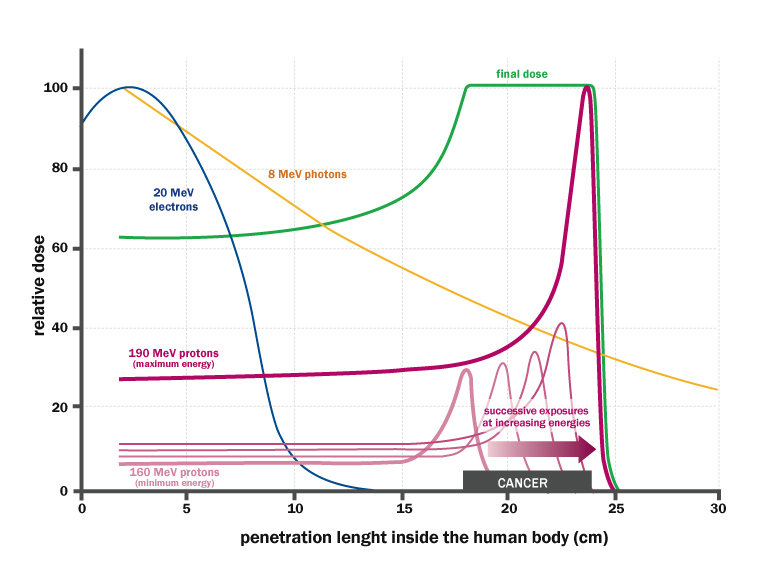
\includegraphics[width=.7\linewidth]{figures/pixel_detectors_usage/Bragg-Peak.png}
            \caption{The Spread Out Bragg Peak (SOBP) curve (green), which is a constant dose distribution, is obtained from the superposition of many Bragg peak of hadrons with different energy.}
            \label{fig:Bragg-peak}
         \end{figure}

        Recently\footnote{The first evidences has been observed on a mice experiments in 1966 and in 2014 by the group of Favaudon and Vozenin. After this, many test on cats and pigs have been performed, and also there has been a clinical trial on a cutaneous tumor-patient} a promising method for RT at ultra high dose rate (at least \SI{40}{Gy/s}) and for this reason called FLASH-RT, instead of CONV-RT (\SI{0.03}{Gy/s}), came out. 
        \begin{table}
            \begin{center}
            \begin{tabular}{|c | c |c |}
            \hline
            & CONV-RT & FLASH-RT \\
            \hline
            \hline
            Dose rate & \SI{0.03}{Gy/s} & \SI{40}{Gy/s}\\
            Intra pulse dose rate & \SI{100}{Gy/s}&\SI{10 6}{Gy/s}\\
            Treatment duration & $\sim$minutes & $\lessapprox$\SI{500}{ms} \\
            DDP & & \SI{1.5}{Gy}\\
            N of pulses & & 10 \\
            \hline
            \end{tabular}
            \caption{\red{Esempi di valori tipici di dose in un trattamento}}
            \label{tab:}
            \end{center}
         \end{table}
        This treatment takes advantages of biological differences between tumors and healthy tissues: it is characterized by reducing normal tissue toxicity and maintaining equivalent tumor damage. 
        The response to dose can be described by the survival fraction probability, describing the fraction of surviving cell as a function of the dose: 
        \begin{multicols}{2}
            \begin{equation}
                S(D) = S(0)\;e^{-F(D)}
            \end{equation}\break
            \begin{equation}
                F(D) = \alpha D \, + \, \beta D^2
            \end{equation}
            \label{eq:survival_curve}
        \end{multicols}
        \red{dove F(D) è una funzione che rappresenta il danno alle cellule ed $\alpha$ and $\beta$ are respectively}
        Hence, at high doses the density of damages increases and the cells repair becomes more difficult. 
        Even if the FLASH effect is not yet completelly understood, it looks like there are two different recipes which are involved:
        \begin{itemize}
            \item the dose rate: come mostrato in figura ad alti dose rate il danno è maggiore.However at lower dose rates and therefore
            longer irradiation time, other effects such as redistribution of cells through the
            cell cycle and cell repopulation can also modify the sparing effect.
            \item oxygen effect:The presence or absence of molecular oxygen O2 within a cell influences
            the biological effect of ionizing radiation: hypoxic cells are very resistant to
            radiation, whereas normal oxygenated cells are highly radiosensitive.
            Cellule che esibiscono hypoxia (cioè cellule che non hanno ossigeno sono radioresistenti); al contrario normoxia e physoxia non lo sono.
            la presenza di ossigeno rende la curva steeper indicando che lo stesso danno si raggiunge a livelli di dose più bassi rispetto al caso senza ossigeno. Dovuto al fatto che sotto la rad le molecole si rompono e se c'è ossigeno (molto elettronegativo) si possono formare dei radicali dannosi.  
        \end{itemize}    
        \begin{figure}[h!]
            \begin{subfigure}{.5\textwidth}
            \centering
            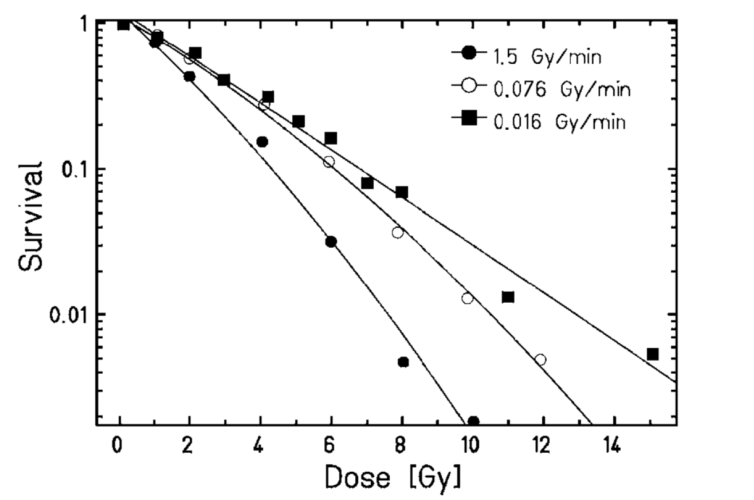
\includegraphics[width=.98\linewidth]{figures/pixel_detectors_usage/survival_curve.png}
            \label{fig:}
            \end{subfigure}
            \begin{subfigure}{.5\textwidth}
                \centering
                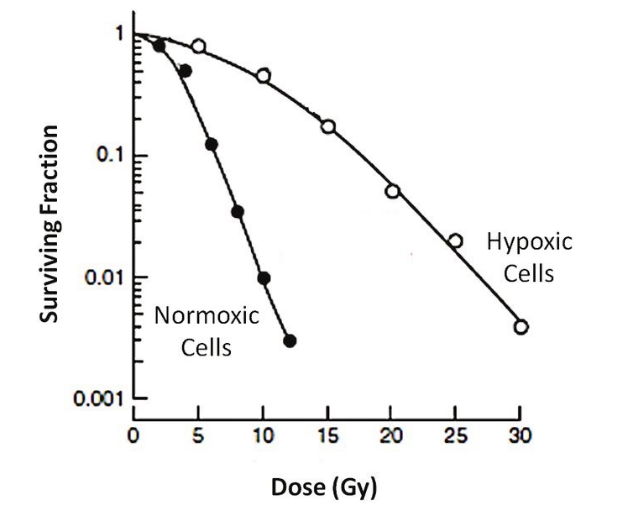
\includegraphics[width=.80\linewidth]{figures/pixel_detectors_usage/survival_curve_oxygen.png}
                \label{fig:survival_curve_oxygen}
            \end{subfigure}
            \caption{(a) Survival curve . (b)}
            \label{fig:}
        \end{figure}

        The Tumor Control Probability (TCP) and the Normal Tissue Complication (NTC) functions parametrize respectively the efficiency of damaging on the tumor after having released a certain dose and the probability of not affecting the healthy tissues. The intermediate zone between the increase of the TC and of the NTC is called therapeutic window, and the wider it is and the more effective the treatment is. 
        \begin{figure}
            \centering
            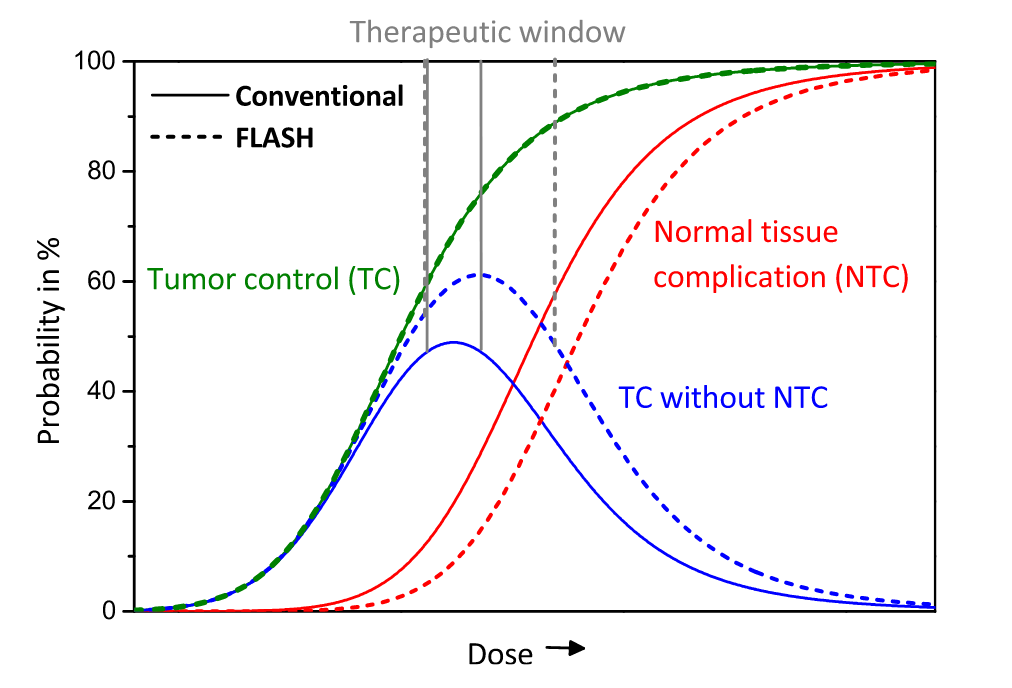
\includegraphics[width=.7\linewidth]{figures/pixel_detectors_usage/curve_flash.png}
            \caption{Illustration of dependence of TCP, NTCP and therapeutic window on dose, for CONV-RT ad FLASH-RT.}
            \label{fig:therapeutic_window}
        \end{figure}

    \subsubsection{Dosimetric problems}
        Finding equipment suitable for dosimetry at ultra high dose rate is an issue: FLASH-RT cause a radical change in the beam characteristics, in the delivery time structure and, above all, in the average and     instantaneous dose-rate, which points-out the limits of the current available dosimeters.
        In fact, the active dosimeters for online monitoring of the beam that are used in daily clinical practice show saturation problem: crucial both for radiobiological studies and for a safe clinical translation.
        On the other hand passive dosimeters could provide dosimetric data, showing dose-rate independence up to 10 alla nove Gy/s for radiochromic films.
        Cosa sono i radiochromic films and they do not have the same accuracy of other detectors.\\
        For online measurements, the available detector are ionization chamber, semiconductors and scintillators, but nevertheless they start to exhibit saturation when the dose-rate/DPP is increased beyond what is used in clinical routine.
        Le camere a ionizzazione hanno già un po' di problemi a DPP di due ordini di grandezza sotto la DDP della flash (quindi quelle tipiche della iort.)
        Doppi problemi sia di saturazione sia di scariche: 
        questo doppio effetto è dato dal fatto che, creandosi tante cariche nella camera, che va ad annullare il campo elettrico di drift. Questo ovviamente paralizza le cariche che non driftano più, ma che anzi si ricombinano ed inoltre facilita la formazione di scariche.
        Scintillators have reusable, non-exhaustible scintillation centers. However, the system has a total deadtime given by both the crystal scintillation time and the electronics read-out deadtime.

        Semiconductors show a nonreversible saturation beyond a threshold around 15 cGy/p. The scintillator used, shows a negligible saturation up to 1 Gy/p, but it increases significantly up to at least 11 Gy/p, and it reaches a cutoff value between 11 and 36 Gy/p.

        Scintillator dosimeters are widely used in radiotherapy. They are usually operating in counting-mode where each detected signal is processed by read-out electronics. When a scintillator dosimeter is used in integrator-mode the signal is integrated over the entire irradiation time.A deadtime, due to the decay time of the scintillating material, is considered on average every N recorded pulses, where N is the number of scintillation centres in the dosimeter.


        Besides saturation i problemi sono anche altri:
        The most important dosimetric aspects needed for an active detector are dose rate independence and high temporal resolution.


        Concerning spatial resolution: Un altro grande limite delle camere a ionizzazione è la risoluzione spaziale dato ch non posson essere fatte più piccole di circa un centimetro. Questo limite è principalmente dovuto a problemi meccanici per cui non si può fare una camera con P bassa e con materiali sottili, perchè le pareti si incurvano. 

        Monitorare la posizione e direzionalità del fascio, anche per la VHEE quindi detto in altre parole un beam monitor.
        Questo detector deve essere abbastanza veloce da poter fornire una risposta in real time e avere anche una buona risoluzione temporale. 

    
    




